\documentclass[12pt]{article}
\usepackage[margin=1.2in]{geometry}
\usepackage[all]{nowidow}
\usepackage[hyperfigures=true, hidelinks, pdfhighlight=/N]{hyperref}
\usepackage{graphicx,amsmath,physics,tabto,float,amssymb,pgfplots,verbatim,tcolorbox}
\usepackage{listings,xcolor,siunitx,subfig,keyval2e,caption,import}
\numberwithin{equation}{section}
\numberwithin{figure}{section}
\definecolor{stringcolor}{HTML}{C792EA}
\definecolor{codeblue}{HTML}{2162DB}
\definecolor{commentcolor}{HTML}{4A6E46}
\lstdefinestyle{appendix}{
    basicstyle=\ttfamily\footnotesize,commentstyle=\color{commentcolor},keywordstyle=\color{codeblue},
    stringstyle=\color{stringcolor},showstringspaces=false,numbers=left,upquote=true,captionpos=t,
    abovecaptionskip=12pt,belowcaptionskip=12pt,language=Python,breaklines=true,frame=single}
\lstdefinestyle{inline}{
    basicstyle=\ttfamily\footnotesize,commentstyle=\color{commentcolor},keywordstyle=\color{codeblue},
    stringstyle=\color{stringcolor},showstringspaces=false,numbers=left,upquote=true,frame=tb,
    captionpos=b,language=Python}
\renewcommand{\lstlistingname}{Appendix}
\pgfplotsset{compat=1.17}

\title{Capacitors}
\date{\textbf{11 August 2020}}
\author{}

\begin{document}

    \begin{titlepage}
        \maketitle
        \center
        \textbf{\large{PHY2004W}}
        \textbf{\large{KDSMIL001}}
        \tableofcontents
    \end{titlepage}
    
    \section{Introduction}
    In this report we will investigate capacitors, specifically in the context of a 
    Resistor-Capacitor (RC) circuit. Firstly we will answer some questions regarding the theory 
    of capacitors and RC circuits, then we will do some experiments and investigate the effects 
    of different frequencies of AC voltage as well as different resistances on the behaviour 
    of RC circuits.

    \section{Theory Questions and Answers}
    \begin{enumerate}
        \item \textbf{Question}: How are $A$, $d$, and $\epsilon$ related, where $A$ is the area of one of the 
        plates in a capacitor, $d$ is the distance between the two plates, and $\epsilon$ is 
        the dielectric constant of the material between the plates. \newline
        \textbf{Answer}: It's fairly easy to see that an increase in the area of the plates of 
        a capacitor $A$ would result in an increase of the amount of charge each plate could hold. 
        This in turn would increase the magnitude of the electric field between each plate and thus 
        increase the potential difference between the plates when fully charged. This results in an 
        increase in capacitance. 
        Similarly the value of $\epsilon$, which is present in the equation for the electric field at 
        a point, will have an effect on the capacitance. Increasing $\epsilon$ results in a decrease 
        in $\vec{E}$ between the plates, allowing for more charge to build up on the plates. 
        Finally, the value of $d$ will also have an inversely proportional effect on the electric 
        field, meaning an increase in $d$ will lead to a decrease in $\vec{E}$ and thus a decrease in 
        the amount of charge able to build up on the plates. 
        This is all summed up in this equation for the capacitance of a capacitor:
        \begin{equation}
            C=\frac{A\epsilon}{d}
            \label{eqn:capacitance}
        \end{equation}
        

        \item \textbf{Question}: By making use of dimensional analysis show that the units of the 
        charging time of a capacitor $\tau$ as given by $\tau = RC$ is seconds (s). \newline
        \textbf{Answer}: $R$ is given by $V/I$, the dimensions of which are 
        \begin{align*}
            &\frac{M^{\frac{1}{2}}L^{\frac{1}{2}}T^{-1}}{M^{\frac{1}{2}}L^{1\frac{1}{2}}T^{-2}} \\
            \implies &L^{-1}T
        \end{align*}
        We also know that $C$ is given by $Q/V$, the dimensions of which are
        \begin{align*}
            &\frac{M^{\frac{1}{2}}L^{1\frac{1}{2}}T^{-1}}{M^{\frac{1}{2}}L^{\frac{1}{2}}T^{-1}} \\
            \implies &L \\
            \implies &[\tau]=[RC]=L^{-1}TL=T
        \end{align*}

        \item \textbf{Question}: Explain what effect an increase and decrease in frequency $\omega$ will have 
        on the reactance and therefore the impedance of the $RC$ circuit. \newline
        \textbf{Answer}: The reactance is given by 
        \begin{equation*}
            X(\omega)=\frac{1}{\omega C}
        \end{equation*}
        meaning that reactance is inversely proportional to the frequency $\omega$. We also know that 
        the impedance of an $RC$ circuit is given by $Z=R+iX(\omega)$. From this we can deduce that 
        an increase in $\omega$ will result in a decrease in $X(\omega)$ which will in turn lead to 
        the impedance being dominated more and more by $R$. As $\omega\rightarrow\infty, Z\rightarrow R$.
    \end{enumerate}

    \section{Practical Questions and Answers}
    \begin{enumerate}\addtocounter{enumi}{3}
        \item \textbf{Question}: What is the correct way to insert a capacitor into a breadboard?
        \newline
        \textbf{Answer}: The correct way to insert a capacitor is Photo C, shown below: 
        \begin{figure}[H]
            \begin{center}
               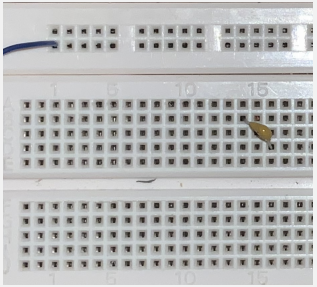
\includegraphics[scale=.5]{PhotoC.png}
               \caption{Photo C}
               \label{fig:Question4Answer}
            \end{center}
        \end{figure}
        \noindent
        The reason for this is the fact that in the other two pictures the capacitor was being short 
        circuited, once by inserting both ends into the same power rail, the long connected pieces at 
        the top and bottom, and once by inserting both ends into the same terminal strip, the shorter 
        vertical pieces.

        \item \textbf{Question}: Why does the charge on the capacitor (or the voltage across it) not 
        reach the same minimum and maximum as the applied signal in the diagram below?
        \begin{figure}[H]
            \begin{center}
               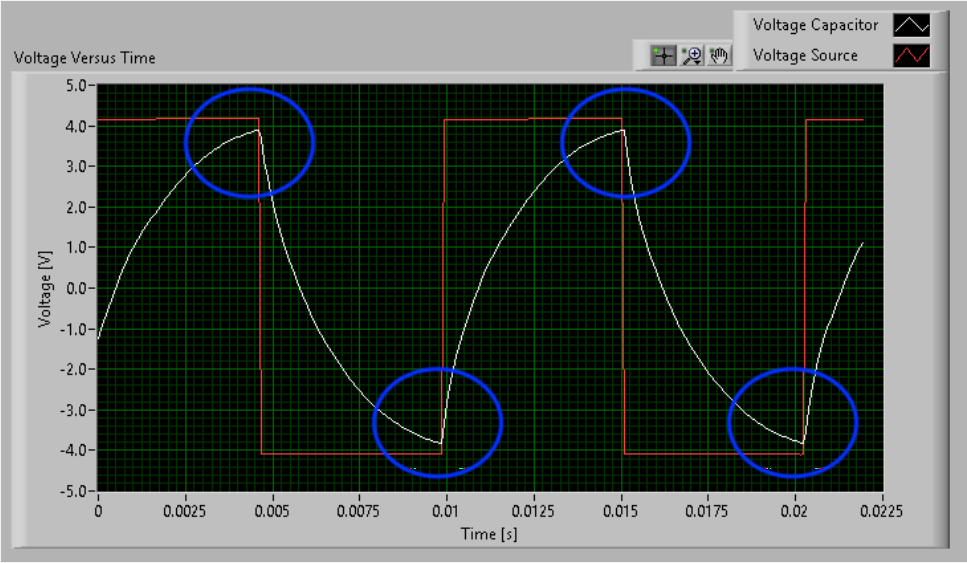
\includegraphics[scale=.5]{Question5Diagram.png}
               \caption{Voltage signal (white) across 100nF capacitor in series with 15 k$\Omega$ resistor}
               \label{fig:Question5Diagram}
            \end{center}
        \end{figure}
        What would you change to ensure the capacitor reaches the same maximum and minimum as the 
        applied signal? \newline
        \textbf{Answer}: The time it takes for a capacitor to reach its full capacity is governed by 
        $\tau = RC$. This means that in order to decrease the time it takes to charge to its theoretical 
        maximum we could decrease either the capacitance of the capacitor or the resistance of the resistor. 
        This could be done by physically changing these components, such as decreasing the surface area of 
        the plates of the capacitor, or simply by swapping out the components for those with a lower value. 
        \newline
        We could also just reduce the frequency of the applied voltage, giving the capacitor more time to 
        charge up before swapping the direction of the current, forcing it to discharge and charge up in 
        the other direction.
    \end{enumerate}

    \section{Data Collecting}
    \subsection{Resistance and Frequency Investigation}
    We were given data in the form of a text file that contained voltage measurements made by the myDAQ. 
    The myDAQ measured the voltage across the 100nF capacitor in an RC circuit as well as across the 
    function generator supplying a square wave voltage with peak-to-peak voltage of $8V_{pp}$. This circuit 
    was set up with 5.6k$\Omega$, 8.2k$\Omega$, and 15k$\Omega$ resistors separately. Each circuit was 
    recorded with 100Hz, 200Hz, 500Hz, and 1000Hz, giving us 12 datasets to work with. This data can be 
    regarded as having a 2\% uncertainty due to the accuracy of the equipment used. We used Python to 
    interpret this data into the plots in \autoref{sec:FreqResistorResponse}, the code for which is in
    % \autoref{code:FreqRes}

    \subsection{Decay Time from the Oscilloscope}
    The figure below is the screen of an oscilloscope measuring the voltage across the frequency generator 
    and the capacitor in an RC circuit with capacitance C=100nF and resistance R=5.6k$\Omega$. We want to 
    determine the time it takes for the capacitor to fully discharge, that is the time difference between 
    the capacitor being at full charge (in this case 4V) and it being at full charge in the "other direction", 
    (having -4V across it).
    \begin{figure}[H]
        \begin{center}
           \includegraphics[width=\textwidth]{Photo2.png}
           \caption{Oscilloscope Display}
           \label{fig:DecayTimeScreen}
        \end{center}
    \end{figure}
    Looking at where the blue line meets the yellow line, it seems to properly come in contact after 17 
    subdivisions, which corresponds to 3.4ms. The measurement has a triangular probability density function, 
    so in order to calculate the uncertainty we use the following formula
    \begin{equation}
        u=\frac{a}{2\sqrt{6}}
    \end{equation}
    where $a$ is the difference between our best upper bound and our best lower bound for the measurement. 
    In our case our best guess could be between 3.2ms and 3.6 ms, so $a=0.4$. This gives us $u=0.081649$.
    That gives us a final measurement of Decay Time = $3.400\pm 0.082$ms. 

    \subsection{Current Measurement}


    \newpage
    \section{Analysis}
    \subsection{Frequency and Resistor Response}\label{sec:FreqResistorResponse}
    Apologies in advance for the small plot size but they are vectorised so you can zoom in as far as you like. 
    \begin{figure}[H]%
        \centering
        \subfloat[100Hz]{\scalebox{0.4}{\subimport{Plots}{Cap_100Hz_5k6.pgf}}}%
        \qquad
        \subfloat[200Hz]{\scalebox{0.4}{\subimport{Plots}{Cap_200Hz_5k6.pgf}}}
        \qquad
        \subfloat[500Hz]{\scalebox{0.4}{\subimport{Plots}{Cap_500Hz_5k6.pgf}}}
        \qquad
        \subfloat[1000Hz]{\scalebox{0.4}{\subimport{Plots}{Cap_1000Hz_5k6.pgf}}}
        \caption{Voltage readings for various frequencies of AC voltage across a 5.6k$\Omega$ resistor}
        \label{fig:5.6kResistor}
    \end{figure}
    
    From the figures above, it's clear to see that an increase in frequency leads to the capacitor not being 
    able to charge up fully in the given time. This makes sense as nothing else in the circuit is changing 
    so the time constant $\tau$ is remaining the same throughout as the time given to the capacitor for it 
    to charge up decreases.
    
    \begin{figure}[H]%
        \centering
        \subfloat[100Hz]{\scalebox{0.4}{\subimport{Plots}{Cap_100Hz_8k2.pgf}}}%
        \qquad
        \subfloat[200Hz]{\scalebox{0.4}{\subimport{Plots}{Cap_200Hz_8k2.pgf}}}
        \qquad
        \subfloat[500Hz]{\scalebox{0.4}{\subimport{Plots}{Cap_500Hz_8k2.pgf}}}
        \qquad
        \subfloat[1000Hz]{\scalebox{0.4}{\subimport{Plots}{Cap_1000Hz_8k2.pgf}}}
        \caption{Voltage readings for various frequencies of AC voltage across a 8.2k$\Omega$ resistor}
        \label{fig:8.2kResistor}
    \end{figure}

    The same is true for the plots above. The resistor in this circuit had a higher resistance and, as 
    we expect from the equation $\tau=RC$, the capacitor couldn't even charge fully at 200Hz, where the 
    circuit with less resistance could. \newline
    \newline
    Below in \autoref{fig:15kResistor} we see exactly the same pattern. A higher resistance leads to the 
    time constant being large and thus the capacitor cannot charge fully in the time given, with it charging 
    less and less per cycle the higher the frequency of the applied voltage.
    
    \begin{figure}[H]%
        \centering
        \subfloat[100Hz]{\scalebox{0.4}{\subimport{Plots}{Cap_100Hz_15k.pgf}}}%
        \qquad
        \subfloat[200Hz]{\scalebox{0.4}{\subimport{Plots}{Cap_200Hz_15k.pgf}}}
        \qquad
        \subfloat[500Hz]{\scalebox{0.4}{\subimport{Plots}{Cap_500Hz_15k.pgf}}}
        \qquad
        \subfloat[1000Hz]{\scalebox{0.4}{\subimport{Plots}{Cap_1000Hz_15k.pgf}}}
        \caption{Voltage readings for various frequencies of AC voltage across a 15k$\Omega$ resistor}
        \label{fig:15kResistor}
    \end{figure}

    \subsection{Time Constant $\tau=RC$}
    In this section we will try to experimentally determine the value of the 

    \newpage
    \section{Appendix}
    \setcounter{figure}{0} \renewcommand{\thefigure}{A.\arabic{figure}}
    % \lstinputlisting[caption=Code that interprets Resistance Frequency data, style=appendix, label=code:FreqRes]{FrequencyResistance.py}
    

\end{document}